%!TEX root = ..\lections.tex
На первой лекции мы уже сталкивались с понятием точечного
отображения. Продолжим знакомство с этим важным и удивительным
объектом нелинейной динамики. Можно выделить два основных сценария
возникновения моделей в виде точечных отображений. Во-первых, для многих
реальных систем характерно изменение их состояний лишь в некоторые
моменты времени. Ясно, что наиболее адекватное описание поведения таких
систем можно получить с помощью моделей с дискретным временем и, в
частности, моделей в форме точечных отображений. Во-вторых, точечные
отображения могут порождаться траекториями динамических систем с
непрерывным временем.

\section{Точечные отображения -- модели дискретных систем}%
\label{sec:6.1}

В настоящее время для управления самыми различными объектами и
процессами широкое распространение получили цифровые автоматические
системы. Такие системы оперируют цифровыми кодами, получаемыми из
непрерывных сигналов путем их квантования по уровню и времени. В
частности, в радиоавтоматике, связи, телевизионных системах,
радиоизмерительных устройствах используются импульсно-фазовые системы
автоподстройки частоты (ИФАП). Как и непрерывная система фазовой
автоподстройки частоты (см. \ref{lect4}), система ИФАП содержит кольцо
авторегулирования. Однако в кольце обратной связи системы ИФАП
используется информация об ошибке, взятая в отдельные моменты времени.
Для этого в типовую структуру схемы ФАП (рис. \ref{fig:4.10}) вводятся
дополнительные элементы: формирующее устройство, преобразующее
синусоидальные сигналы генераторов в короткие импульсы, запоминающее
устройство, фиксирующее выходное напряжение фазового детектора, который
является импульсным, в промежутке между соседними импульсами. Типовая
система ИФАП с идеальным запоминанием и отсутствием фильтра в цепи
управления описывается уравнением
\begin{equation}
        \label{eq:6.1}
        \phi(n+1) - \phi(n) + \alpha F( \phi(n)) = \gamma.
\end{equation}
Уравнение \eqref{eq:6.1} связывает разность фаз $\phi$ сигнала подстраиваемого генератора
и опорного сигнала в соседние моменты времени $n$ и $n+1$, где $n = 1,2,3,\dots$
соответствует моментам времени $t=n \tau_0$, а $\tau_0$--период дискретизации.
В \eqref{eq:6.1} $F( \phi)$-- $2 \pi$-периодическая функция --
 характеристика фазового дискриминатора,
нормированная на единицу,
$\gamma = \Omega_H \tau_0$
-- параметр пропорциональный
начальной расстройке
$\Omega_H$ генераторов, $\alpha = \Omega \tau_0$
-- параметр цепи управления.
В силу инвариантности уравнения \eqref{eq:6.1} относительно преобразования
$\phi \to \phi + 2 \pi$ , оно представляет собой точечное отображение окружности на
себя.

Другими примерами реальных процессов, которые адекватно
описываются точечными отображениями, могут служить колебания
численности биологических популяций. Например, динамика некоторых
популяций в замкнутой среде достаточно хорошо описывается (П.Ф.
Ферхюльстом, 1845) так называемым логистическим отображением
\begin{equation}
        \label{eq:6.2}
        x(n+1) = \mu x(n) (1- x(n)),
\end{equation}
где $x(n)$ -- нормированная численность особей в $n$-й год, а $\mu$ -- параметр, зависящий от плодовитости особой
в $(n+1)$-й год -- $x(n+1)$ пропорциональна численности в предыдущий год --
$x(n)$ и свободной части жизненного пространства, которая в свою очередь пропорциональная величине $(1 - x(n))$.

\section{Отображение Пуанкаре}%
\label{sec:6.2}

Как мы уже отмечали,  в некоторых случаях точечные отображения могут
генерироваться траекториями динамических систем с непрерывным временем.
Такие отображения называют \textbf{отображениями Пуанкаре} . Поясным процедуру
возникновения отображения Пуанкаре на простейшем примере. Рассмотрим
систему с непрерывным временем вида
\begin{equation}
        \label{eq:6.3}
        \begin{cases}
                \dot x = y,
                \dot y = -2 \delta y - \omega_0^2 x,
        \end{cases}
\end{equation}
где $\delta$ и $\omega_0$--положительные параметры. 
Система \eqref{eq:6.3} описывает динамику
линейного осциллятора с диссипацией (см. \ref{lect5}). Пусть $\omega_0^2>\delta^2$ . В этом
случае на фазовой плоскости системы \eqref{eq:6.3} существует единственное
устойчивое состояние равновесия в начале координат -- устойчивый фокус,
который притягивает все остальные траектории системы (рис. \ref{fig:6.1}а). Покажем,
что траектории системы \eqref{eq:6.3} порождают одномерное точечное отображение
полупрямой $N = \qty{y=0, ~ x<0}$ на себя. Запишем общее решение системы \eqref{eq:6.3}
\begin{equation}
        \label{eq:6.4}
        \begin{cases}
                x(t) = e^{-\delta t} \qty[ C_1 \cos(\omega t) + C_2 \sin(\omega t) ],\\
                y(t) = e^{-\delta t} \qty[ (C_2 \omega - \delta C_1) \cos(\omega t) - (C_2 \delta + C_1 \omega) \sin( \omega t) ],  
        \end{cases}
\end{equation}
где $\omega = \sqrt{ \omega_0^2 - \delta ^2}$, $C^{1,2}$ -- произвольные константы. Рассмотрим траекторию $L$,
выходящую при $t=0$ из некоторой произвольной точки с координатами $x=x_{0}$ 
$(x_0>0)$, $y=0$ (см. рис.\ref{fig:6.1}а). Из \eqref{eq:6.4} получаем уравнение траектории $L$ 
\begin{equation}
        \label{eq:6.5}
        \begin{cases}
                x(t) = e^{-\delta t} x_0 \qty[ \cos(\omega t) + \frac{\delta}{\omega} \sin(\omega t) ],
                y(t) = e^{- \delta t} x_0 \qty( \frac{\delta^2}{\omega} + \omega)   \sin(\omega t).
        \end{cases}
\end{equation}

\begin{figure}[h]
        \centering
        \begin{minipage}{0.49\linewidth}
                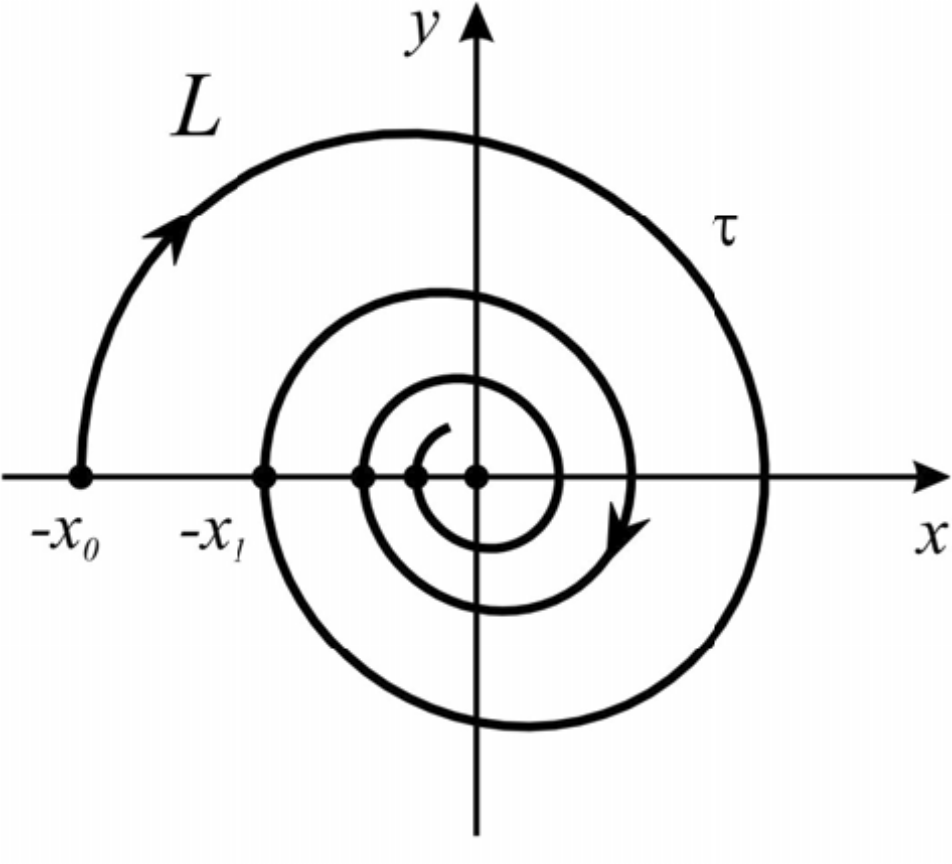
\includegraphics[width=\linewidth]{fig/lect6/1a}
        \end{minipage}
        \begin{minipage}{0.49\linewidth}
                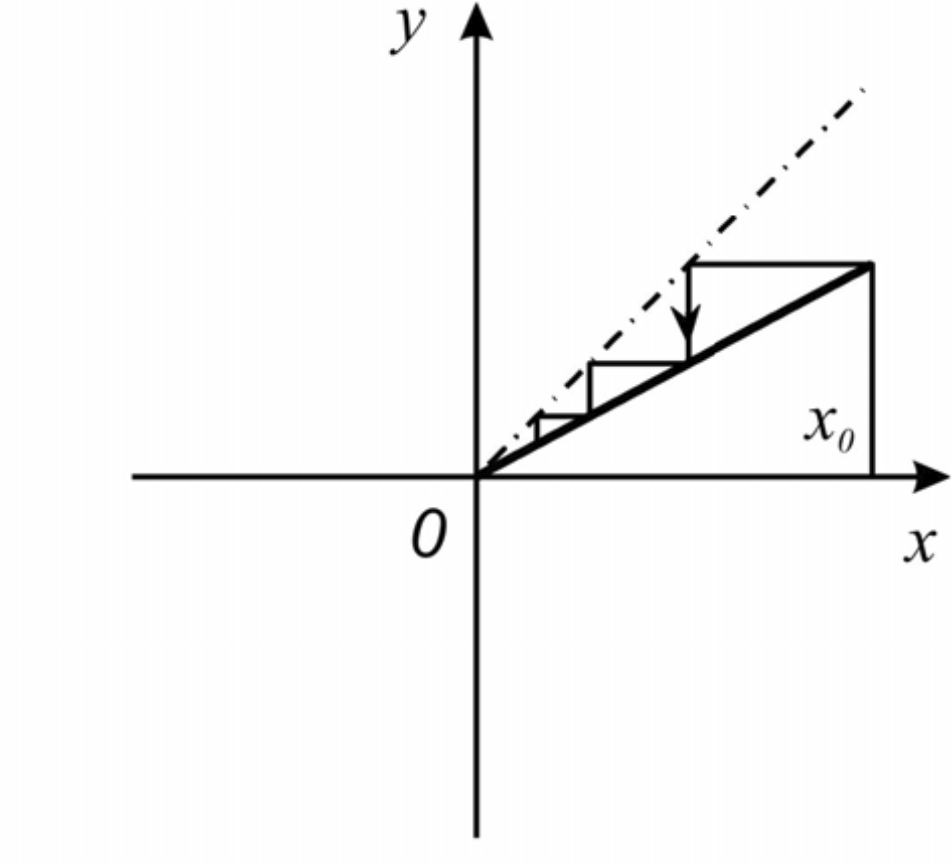
\includegraphics[width=\linewidth]{fig/lect6/1b}
        \end{minipage}
        \caption{Фазовый портрет системы \eqref{eq:6.3} (а); отображение Пуанкаре \eqref{eq:6.8} (b).}
        \label{fig:6.1}
\end{figure}
Найдём координату точки, в которой $L$ первый раз пересекает полупрямую $N$. Обозначим через $\tau$ время движения по траектории $L$ между этой и начальной точками. Тогда координаты искомой точки можно найти из условий
\begin{equation}
        \label{eq:6.6}
        y(\tau) = 0, \quad x(\tau) = - x_1.
\end{equation}
Из \eqref{eq:6.6}, используя \eqref{eq:6.5}, получаем
\begin{equation}
        \label{eq:6.7}
        \tau = \frac{2 \pi}{\omega} \text{ и } x_1 = e^{-\delta \frac{2 \pi}{\omega}} x_0. 
\end{equation}
Поскольку точка $x_0$ была произвольной, уравнение \eqref{eq:6.7} задает преобразование любой точки полупрямой $N$, т.е. искомое точечное отображение
\begin{equation}
        \label{eq:6.8}
        \bar x = e^{- \delta \frac{ 2 \pi}{\omega}} x.
\end{equation}
Отображение \eqref{eq:6.8} – линейное точечное отображение. Качественный вид
отображения представлен на рис. \ref{fig:6.1}b. Его динамика чрезвычайно проста –
любая траектория отображения асимптотически приближается к значению $x=0$.
Прямая $N$, на которой определено отображение Пуанкаре, называется \textbf{секущей
Пуанкаре} (термин <<секущая>> отражает наличие потока траекторий,
проходящего через нее).

Рассмотренный пример показывает, что для секущей Пуанкаре характерны следующие свойства
\begin{itemize}
        \item возвращаемость траекторий;
        \item во всех точках траекторий пресекают секущую так, что наклон касательных к ним в этих точках не равен нулю (такое пересечение называется трансверсальным см. лекцию \ref{lect1}.
\end{itemize}
Заметим, что секущей Пуанкаре может быть не обязательно прямая, а,
например, некоторая кривая (для систем на плоскости), на которой
выполняются вышеперечисленные свойства. Очевидно, что в общем случае
размерность секущей Пуанкаре на единицу меньше размерности фазового
пространства динамической системы. Например, для систем с трехмерным
фазовым пространством это двумерная поверхность. Секущая Пуанкаре может
быть как локальной, когда ее пересекает лишь часть траекторий, так и
глобальной, когда ее пересекают все траектории динамической системы
(например, как в случае системы \eqref{eq:6.3}). Заметим также, что отображение
Пуанкаре существует далеко не всегда. Например, если на фазовой плоскости
существует единственное состояние равновесия \textbf{седло} , с сепаратрисами,
уходящими в бесконечность, то отображение Пуанкаре не существует.

Однако, существует важный класс динамических систем, для которого
секущая Пуанкаре всегда существует и, более того, является глобальной. Это
неавтономные системы с периодической правой частью (например, системы,
находящиеся под действием периодического внешнего силового воздействия).
Поясним ситуацию на примере неавтономной системы второго порядка
\begin{equation}
        \label{eq:6.9}
        \begin{cases}
                \dot x_1 = f_1 (x_1,x_2,t) \\
                \dot x_2 = f_2 (x_1,x_2,t), 
        \end{cases}
\end{equation}
где $f_i(x_1,x_2,t)$-- периодические функции с периодом $T = \frac{2 \pi}{\omega}.$ Сделав в \eqref{eq:6.9} замену $t = \frac{\theta}{\omega}$, получим систему
\begin{equation}
        \label{eq:6.10}
        \begin{cases}
                \dot x_1 = f_1 \qty( x_1,x_2, \frac{\theta}{\omega}),\\
                \dot x_2 = f_2 \qty(x_1,x_2, \frac{\theta}{\omega}), \\
                \dot \theta = \omega.\\
        \end{cases}
\end{equation}
Система \eqref{eq:6.10} -- автономная система третьего порядка, не имеющая
состояний равновесия в силу того, что $\dot \theta = \omega>0$. Отсюда также следует, что люьая траектория системы \eqref{eq:6.9}, <<стартующая>> с плоскости 
$\Sigma = \qty{ t =t_0=\const, ~ ( x_1,x_2) \in \R^2}$, за конечное время придёт на плоскость
$\Sigma = \qty{ t=t_0 + \frac{2\pi}{\omega}, ~ (x_1,x_2) \in \R^2}$ (см. рис.\ref{fig:6.2}).
\begin{figure}[h]
        \centering
        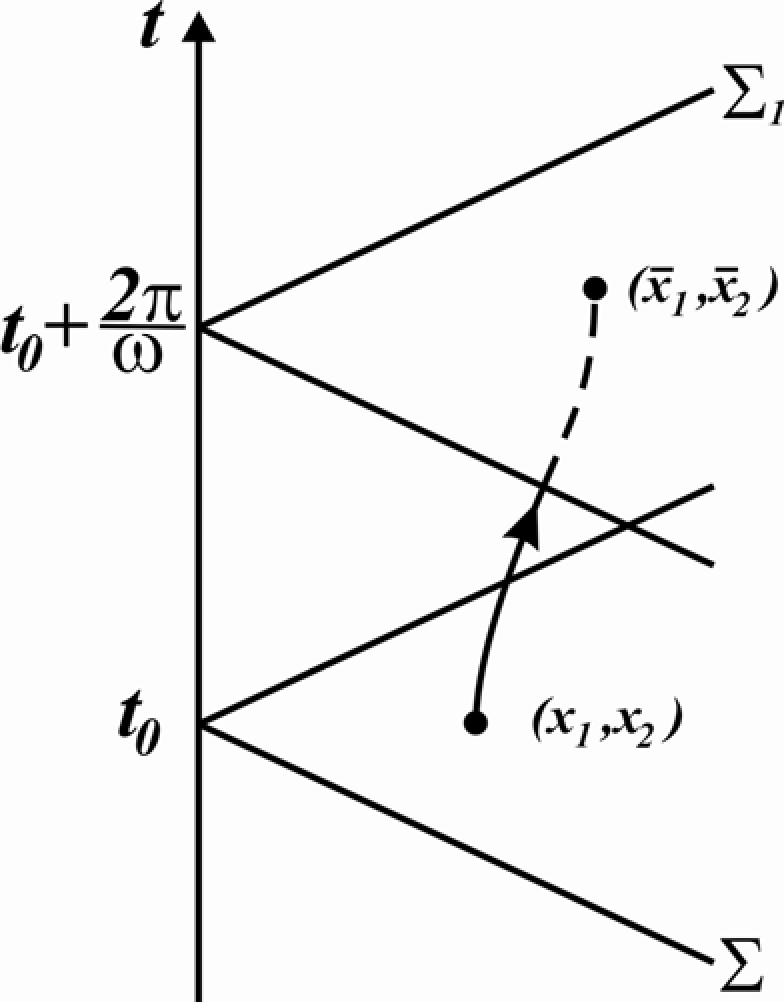
\includegraphics[]{fig/lect6/2}
        \caption{Генерация отображения Пуанкаре системой \eqref{eq:6.9}}
        \label{fig:6.2}
\end{figure}
В силу периодичности правых частей системы \eqref{eq:6.9} плоскости
$\Sigma$ и $\Sigma_1$ тождественны и, следовательно, систему \eqref{eq:6.9} порождает двумерное точечное отображение
\begin{equation}
        \label{eq:}
        P: \quad \Sigma \to \Sigma.
\end{equation}

Конечно, рассмотренный выше простейший пример (система \eqref{eq:6.3})
введения отображения Пуанкаре не позволяет в полной мере судить о
целесообразности такой процедуры. Однако, позднее на более содержательных
примерах мы покажем, что исследование динамических систем с помощью
отображения Пуанкаре является одним из эффективных методов современной теории колебаний.

Перейдем к изучению свойств точечных отображений.

\section{Неподвижные точки}%
\label{sec:6.3}

Рассмотрим $m$-мерное нелинейное точечное отображение
\begin{equation}
        \label{eq:6.11}
        \bar{ \vec x} = \vec F(\vec x), ~ \vec x \in \R^m, ~ \vec F: \R^m \to \R^m.
\end{equation}
Напомним, что в \eqref{eq:6.11} $ \bar{\vec x} = \vec x (n+1)$, а  $\vec x \equiv \vec x(n)$, а $n$-- дискретное время. Аналогично случаю динамических систем с непрерывным временем, для системы \eqref{eq:6.11} также можно ввести понятие полутраектории и траектории, которые задаются соответственно следующим образом
\begin{equation}
        \label{eq:}
        \qty{ \vec F^n \vec x_0}_{n=0}^{+\infty}
        \text{ и }
        \qty{ \vec F^n \vec x_0}_{n=-\infty}^{+\infty},
\end{equation}
где $\vec x_0 = \vec x(0)$. Очевидно, что в фазовом пространстве системы \eqref{eq:6.11}
они
представляют собой последовательности точек. Простейшим видом траекторий
системы  \eqref{eq:6.11} являются так называемые неподвижные точки. Неподвижными
точками отображения  \eqref{eq:6.11} называются такие значения $x$ , которые не
изменяются под его действием, т.е. являются решениями системы
\begin{equation}
        \label{eq:6.12}
        \vec x = \vec F( \vec x).
\end{equation}
Пусть $\vec x = \vec x^*$ -- решение системы  \eqref{eq:6.12} и, следовательно, $\vec x = \vec x^*$ --
одна из неподвижных точек отображения  \eqref{eq:6.11}. Для неподвижных точек, аналогично состояниям равновесия
конечномерных систем с непрерывным временем
может быть введено понятие устойчивости по Ляпунову. Незначительное
различие состоит в дискретности времени и траекторий, Далее, говоря об
устойчивости неподвижных точек, мы будем понимать их устойчивость в
смысле Ляпунова. Запишем отображение \eqref{eq:6.11} в новых переменных
\begin{equation}
        \label{eq:6.13}
        \vec \xi = \vec x - \vec x^*
\end{equation}
Из \eqref{eq:6.11} и \eqref{eq:6.13} имеем
\begin{equation}
        \label{eq:6.14}
        \vec x^* + \bar{ \vec \xi} = \vec F \qty( \vec x^* + \vec \xi).
\end{equation}
Разлагая правые части системы \eqref{eq:6.14} в степенные ряды по $\vec \xi$, приходим к линейному 
$m$-мерному отображению
\begin{equation}
        \label{eq:6.16}
        \bar{\vec{\xi}} = \vec A \vec{\xi},
\end{equation}
где $\vec A$--постоянная $m \times m$-матрица с элементами $\displaystyle a_{ik} = \pdv{f_i}{x_k} \eval_{x=x^*}$. Будем искать решение системы \eqref{eq:6.16} в виде
\begin{equation}
        \label{eq:6.17}
        \vec{\xi}(n) = \vec C (s)^n,
\end{equation}
где $\vec C$ -- постоянный вектор столбец. Подставляя \eqref{eq:6.17} в \eqref{eq:6.16}, получим характеристический определитель
\begin{equation}
        \label{eq:6.18}
        \det(\vec A - s \vec E) = 0,
\end{equation}
где $\vec E$-- единичная $m \times m$-матрица. Раскрывая определитель \eqref{eq:6.18}, приводим к характеристическому уравнению. Корни этого уравнения, которые обозначим через $s_{i},~ i=1,2,\dots,m,$ называются \textbf{мультипликаторами} неподвижной точки $\vec x = \vec x^*$.

На предыдущей лекции мы отмечали, что структура траекторий в
окрестности грубого состояния равновесия топологически эквивалентна ее
линеаризации. Аналогичное утверждение справедливо и для неподвижных
точек. Именно, если мультипликаторы неподвижной точки удовлетворяют
условию  $|s_i| \neq 1,~ i=1,2,\dots,m,$, то она является грубой (структурно устойчивой) и
существует гомеоморфизм, который переводит каждую траекторию из
достаточно малой окрестности неподвижной точки нелинейного отображения
\eqref{eq:6.11} в траекторию из окрестности соответствующей неподвижной точки
линейного отображения \eqref{eq:6.16} с сохранением направления движения.
Следовательно, грубые неподвижные точки отображения \eqref{eq:6.11} могут быть
исследованы на устойчивость и классифицированы с помощью
соответствующих линейных отображений. В частности, из \eqref{eq:6.17} следует, что
неподвижная точка
$\vec x = \vec x^*$ отображения \eqref{eq:6.11} будет асимптотически
устойчивой $n \to + \infty$ , если все ее мультипликаторы
$s_i$ 
 на комплексной
плоскости лежат строго внутри единичной окружности, т.е. удовлетворяют
условию
\begin{equation}
        \label{eq:6.19}
        |s_i| < 1, i = 1,2,\dots,m.
\end{equation}
Если же среди мультипликаторов $s_i$ существует хотя бы один расположенный на комплексной плоскости вне единичной окружности, то неподвижная точка $\vec x = \vec x^*$ отображения \eqref{eq:6.11} неустойчива по Ляпунову.

\section{Одномерные линейные отображения}%
\label{sec:6.4}

Рассмотрим отображения \eqref{eq:6.16} в одномерном $(m=1)$ случае 
\begin{equation}
        \label{eq:6.20}
        \bar{\xi} = a \xi, 
\end{equation}
где $a$- параметр, $a\neq 0$. Предположим сначала, что $a \neq 1$. Очевидно, что $\xi=0$--
неподвижная точка отображения \eqref{eq:6.20}. Будем искать решение уравнения \eqref{eq:6.20} в виде \eqref{eq:6.17}. Подставляя \eqref{eq:6.17} в \eqref{eq:6.20} находим, что мультипликатор $s = a$. Следовательно, неподвижная точка $\xi=0$ является асимптотически устойчивой, если
$|a|<1$ и неустойчивой, если $|a|>1$.

Рассмотрим как переменная $\xi(n)$ изменяется во времени $n$ под действием отображения \eqref{eq:6.20} при различных значениях параметра.

В случае одномерных отображений (отображение \eqref{eq:6.11} в случае $m=1$ ) и, в частности, отображения \eqref{eq:6.20}, эволюцию $\xi(n)$ удобно изучать с помощью так называемой 
\textbf{диаграммы Ламерея}. 
 Отображение рассматривается не в фазовом
пространстве, которое является одномерным, а на вспомогательной плоскости
$(x,\bar x)$. На этой плоскости каждой траектории отображения соответствует
некоторая ломаная линия, которая строится следующим образом. Прежде всего,
на плоскости $(x,\bar x)$ проводится построение графика функции $F(x)$, которую
называют \textbf{функцией последования}. При этом точки пересечения этого графика
с биссектрисой $\bar x = x$ соответствуют неподвижным точкам отображения. Затем
из точки на оси абсцисс, соответствующей начальному условию
$x_0$,
несовпадающему с координатами неподвижных точек, проводится
вертикальная прямая до пересечения с графиком функции последования $F(x)$ .
Ордината найденной таким образом точки соответствует значению 
$x(1) = F(x_0)$.
Далее из этой точки проводится горизонтальная прямая до пересечения с
биссектрисой. Тем самым устанавливается новая начальная точка на оси
абсцисс для нахождения следующей итерации отображения, т.е.  $x(2)=F(x(1))$ .
Затем процедура повторяется и на плоскости $(x,\bar x)$, формируется некоторая
ломаная линия.

На рис. \ref{fig:6.3} представлены диаграммы Ламерея отображения \eqref{eq:6.16} для
различных значений параметра $a$ и отвечающие им временные реализации
переменной  $\xi(n)$.

Заметим, что в случае $a<0$ на диаграмме Ламерея при каждой итерации
изображающая точка меняет свое расположение относительно неподвижной
точки и изменение переменной $\xi$ во времени имеет немонотонный характер.
При этом, если $a=-1$ , все траектории отображения \eqref{eq:6.20} являются
периодическими с периодом 2 (рис.\ref{fig:6.3} d). Действительно, в этом случае при
любом начальном условии $\xi(0) ~ (\xi(0) \neq 0)$ траектория возвращается в него через
две итерации. Наконец, обратим внимание на то, что при $a=1$ отображение
\eqref{eq:6.20} является вырожденным и имеет континуум неподвижных точек.
\begin{figure}[h]
        \centering
        \caption{Диаграмма Ламерея для отображения \eqref{eq:6.20} и соответствующая
        эволюция переменной $\xi(n)$ в случае $0<a<1$ (a); в случае
$-1<a<0$ (b); в случае $a>1$ (c); в случае $a<-1$ (d); в случае $a=-1$ (e).}
        \label{fig:}
\end{figure}

\section{Двумерные линейные отображения}%
\label{sec:6.5}

При $m=2$ отображение \eqref{eq:6.16} принимает вид
\begin{equation}
        \label{eq:6.21}
        \begin{cases}
                \bar \xi_1 = a \xi_1 + b \xi_2,
               \bar \xi_2 = c\xi_1+ d\xi_2,
        \end{cases}
\end{equation}
где $a,b,c,d$ - некоторые параметры, а характеристическое уравнение, определяющее мультипликаторы $s_{1,2}$ неподвижной точки $O(\xi_1=\xi_2=0)$, записывается следующим образом
\begin{equation}
        \label{eq:6.22}
        s^2 - (a+d) s + (ad-bc) = 0.
\end{equation}
Проведем классификацию возможных типов неподвижной точки $O$, считая, что её мультипликаторы не лежат на единичной окружности, т.е. $|s_{1,2}| \neq 1$.

\subsection{Действительные мультипликаторы}%
\label{sub:6.5.1}

Предположим, что уравнение \eqref{eq:6.22} имеет действительные мультипликаторы и выполнено условие $s_1 \neq s_2$. В этом случае, аналогично случаю линейных динамических систем с непрерывным временем, линейным невырожденным преобразованием координат (см. лекцию \ref{lect3}) система \eqref{eq:6.21} преобразуется к виду
\begin{equation}
        \label{eq:6.23}
        \begin{cases}
                \bar u_1 = s_1 u_1,
               \bar u_2 = s_2 u_2. 
        \end{cases}
\end{equation}
Система \eqref{eq:6.23} -- нормальная форма уравнений грубой неподвижной точки с действительными мультипликаторами. Рассмотрим решение системы \eqref{eq:6.23} с начальными условиями $u_1(0)=u_1^0$,$u_2(0) = u_2^0$ :
\begin{equation}
        \label{eq:6.24}
        u_1(n)  = u_1^0 (s_1)^n,\\
        u_2(n) = u_2^0(s_2)^n.
\end{equation}
Непосредственно из \eqref{eq:6.24} вытекают следующие свойства отображения \eqref{eq:6.23}.
\begin{itemize}
        \item Если $|s_{1,2}| <1$, то при любых начальных условиях $u_1^0$, $u_2^0$ 
                \begin{equation}
                        \label{eq:}
                        \lim_{n \to \infty} u_i(n) = 0, \quad i=1,2
                \end{equation}
                и неподвижная точка $O$ является асимптотически устойчивой.
        \item Если $|s_1|<1, ~ |s_2|>1$ или $|s_1|>1,~ |s_2|<1$, то неподвижная точка $O$ 
                        является седловой.
        \item Если $|s_{1,2}|>1$, то при любых нетривиальных начальных условиях $u_1^0$, $u_2^0$ 
                имеем
                \begin{equation}
                        \label{eq:}
                        \lim_{n \to \infty} u_i(n) = \infty,\quad i=1,2
                \end{equation}
                и неподвижная точка $O$ является неустойчивой.
\end{itemize}

Рассмотрим возможные фазовые портреты отображения \eqref{eq:6.23} Ограничимся случаем выполнения условия $s_1 \cdot s_2 >0$, представляющим наибольший интерес, поскольку этому условию удовлетворяют
мультипликаторы неподвижных точек отображений Пуанкаре.

\subsubsection{Неподвижная точка устойчивый узел}%

Как было показано выше, для устойчивости неподвижной точки ее
мультипликаторы на комплексной плоскости должны быть расположены
внутри единичной окружности. В случае действительных мультипликаторов
возможны два (при выполнении $s_1 \cdot s_2>0$ ) варианта такого расположения.

\paragraph{Положительные мультипликаторы. $1>s_1>s_2>0$.}%

Получим уравнение фазовых кривых отображения \eqref{eq:6.23} в этом случае. 
Для этого возведем первое уравнение в системе \eqref{eq:6.24} в степень $\lg s_2$, а второе --
в степень $\lg s_1$. В результате получим
\begin{equation}
        \label{eq:6.25}
        \begin{cases}
                (u_1(n))^{\lg s_2} = (u_1^0)^{\lg s_2} (s_1)^{n \lg s_2} \\
                 (u_2(n))^{\lg s_1} = (u_2^0)^{\lg s_1} (s_2)^{n \lg s_1}.
        \end{cases}
\end{equation}
Поскольку
\begin{equation}
        \label{eq:6.26}
        ( u_2(n))^{\lg s_1} = C\qty( u_1(n) )^{\lg s_2},
\end{equation}
где
\begin{equation}
        \label{eq:}
        C = \frac{( u_2^0)^{\lg s_1}}{(u_1^0)^{\lg s_2}}.
\end{equation}
Из \eqref{eq:6.25} следует, что в рассматриваемом случае все траектории, за исключением траекторий, отвечающих значениям
$C=0$ и $C=\infty$, имеют параболический вид и касаются в начале координат ось абсцисс, поскольку
\begin{equation}
        \label{eq:}
        \dv{u_2}{u_1} \eval_{u_1=0} = 0.
\end{equation}
При $C=0$ и $C=\infty$, фазовые кривые выражаются в прямые 
$\qty{u_2=0}$ и $\qty{u_{1}=0}$ соответственно. Из
\eqref{eq:6.26} следует, что любая нетривиальная траектория системы 
системы  \eqref{eq:6.23} асимптотически приближается к неподвижной  точек, которая называется
\textbf{устойчивым узлом} (см. рис.\ref{fig:6.4}), а прямые $\qty{u_2=0}$ и $\qty{u_1=0}$
его \textbf{ведущим} и \textbf{неведущим} направлениями.

\paragraph{Отрицательные мультипликаторы. $-1<s_1<s_2<0$.}%

В этом случае
свойства неподвижной точки O аналогичны предыдущему случаю, и она также
называется устойчивым узлом. Однако, стремление траекторий к неподвижной
точке имеет специфику, связанную с тем, что ее мультипликаторы
отрицательны. Благодаря этому, при каждой итерации изображающая точка
изменяет знак своих координат на противоположный. Другими словами,
траектории стремятся к неподвижной точке, поочередно перескакивая на
фазовой плоскости
$(u_1,u_2)$ с одной фазовой кривой на другую. Однако, через
одну итерацию изображающая точка вновь возвращается на первоначальную
фазовую кривую, т.е. траектории отображения второй степени задаются тем же
уравнением \eqref{eq:6.26}, в котором $s_1$ и $s_2$ нужно формально заменить на
$s_1^2$ и $s_2^2$
соответственно.

\paragraph{Неподвижная точка неустойчивый узел}%

Рассмотрим свойства отображений \eqref{eq:6.23}, когда оба мультипликатора расположены вне единичной окружности.
Здесь, как и в предыдущем случае, они могут быть как положительными (см. рис.\ref{fig:6.4}с), так и отрицательными (см. рис.\ref{fig:6.4}d). В обоих случаях в силу \eqref{eq:6.24} траектории отходят от неподвижной точки и, следовательно, она неустойчива. Такая неподвижная точка называется 
\textbf{неустойчивым узлом}. Фазовые кривые на плоскости по-прежнему задаются уравнением \eqref{eq:6.26}, по которым траектории отходят от неподвижной точки.

\paragraph{Неподвижная точка седло}%

Пусть неподвижная точка $O$ имеет один мультипликаторы вне, а второй -- внутри единичной окружности, т.е. $s_1,s_1$ удовлетворяют условиям: $0<s_1<1<s_2$ (см. 
\label{par:nepodvizhnaia_tochka_sedlo}


Пусть неподвижная точка $O$ имеет один мультипликаторы вне, а второй --
внутри единичной окружности, т.е.
$s_1,s_2$ удовлетворяют условиям:
$0 < s_1 <1<s_2$
(рис. \ref{fig:6.4}e) или 
$s_2<-1<s_{1}<0$(рис.\ref{fig:6.4}f). По-прежнему прямые
$\qty{u_2=0}$ и $\qty{u_1=0}$ 
u являются инвариантными. Прямая $\qty{u_2=2}$ 
 состоит из $O$ и
двух траекторий асимптотически стремящихся к ней, а прямая 
$\qty{u_1=0}$
включает в себя, кроме неподвижной точки $O$, две траектории, уходящие от
нее. Такая неподвижная точка называется седлом . Две приближающиеся к ней
траектории называются устойчивыми, а две удаляющиеся траектории –
неустойчивыми сепаратрисами неподвижной точки $O$. Заметим, что уравнение
\eqref{eq:6.26} остается справедливым в рассматриваемом случае и показывает, что все
траектории отображения, кроме сепаратрис, имеют вид гипербол, которые
проходят мимо $O$ (рис. \ref{fig:6.4}e,f). При этом в случае отрицательных
мультипликаторов изображающая точка двигается по траекториям со скачками.
Пример такого движения показан на рис.\ref{fig:6.4}f  пунктирной линией. Обратим
внимание, что на фазовой плоскости
$(\xi_1,\xi_2)$
 исходной системы \eqref{eq:6.21}
сепаратрисы cедловой неподвижной точки имеют в общем случае вид прямых,
не обязательно совпадающих с осями координат, как это имеет место для
плоскости $(u_1,u_2)$. 

\subsection{Комплексные мультипликаторы}%

Предположим, что неподвижная точка $O$ имеет косплексно-сопряженные мультипликаторы
\begin{equation}
        \label{eq:6.27}
        s_{1,2} = \alpha \pm i \beta.
\end{equation}
В этом случае переменные $u_1$ и $u_2$ в \eqref{eq:6.23} являются комплексными, т.е.
\begin{gather}
        u_1 = u + iv, \\
        u_2 = u - iv. \\
\end{gather}
Подставляя \eqref{eq:6.27}, \eqref{eq:6.28} в \eqref{eq:6.23}, получим
\begin{equation}
        \label{eq:6.29}
        \begin{cases}
                \bar u + i \bar v = (\alpha + i\beta)(u+ i v),\\
                \bar u - i \bar v = (\alpha - i \beta)(u-iv),
        \end{cases}
\end{equation}
Из \eqref{eq:6.29} находим
\begin{equation}
        \label{eq:6.30}
        \begin{cases}
                \bar u = \alpha u - \beta v,
                \bar v = \beta u + \alpha v.
        \end{cases}
\end{equation}
Система \eqref{eq:6.30} является нормальной формой уравнений грубой неподвижной точки
с комплексно-сопряженными мультипликаторами. Исследуем свойства фазовых траекторий системы 
\eqref{eq:6.30}. Представим мультипликаторы $s_{1,2}$ в тригонометрическом виде
\begin{equation}
        \label{eq:}
        s_{1,2} = |s|( \cos \omega \pm i \sin \omega),
\end{equation}
где
\begin{equation}
        \label{eq:6.31}
        |s| = \sqrt{\alpha^2 + \beta^2}, \quad \alpha = |s| \cos \omega, \quad \beta=|s|\sin \omega.
\end{equation}
При использовании \eqref{eq:6.31} система \eqref{eq:6.30} преобразуется к виду
\begin{equation}
        \label{eq:6.32}
        \begin{cases}
                \bar u = |s| (u\cos \omega - v \sin \omega),\\
                \bar v = |s|(u\sin \omega + v \cos \omega). 
        \end{cases}
\end{equation}
Переходя в системе \eqref{eq:6.32} к полярным координатам
\begin{equation}
        \label{eq:}
        u = \rho \cos \phi, \quad v = \rho \sin \phi,
\end{equation}
получим
\begin{equation}
        \label{eq:6.33}
        \begin{cases}
                \bar \rho \cos \bar \phi = |s| ( \rho \cos \omega \cdot \cos \phi - \rho \sin \omega \cdot \sin \phi) = |s| \rho \cos(\phi+w) \\
                \bar \rho \sin \bar \phi = |s| (\rho\sin \omega \cdot \cos \phi + \rho \cos \omega \cdot \sin \phi) = |s| \rho \sin(\phi+w).
        \end{cases}
\end{equation}
Разрешая систему \eqref{eq:6.33} относительно $\bar \rho$ и $\bar \phi$, находим
\begin{equation}
        \label{eq:6.34}
        \begin{cases}
                \bar \phi = \phi + \omega ,\\
                \bar \rho = |s| \rho.
        \end{cases}
\end{equation}
В системе \eqref{eq:6.34} уравнения для переменных $\phi$ и $\rho$ независимы, что позволяет легко
найти их решение и получить вид траекторий отображения
\begin{equation}
        \label{eq:6.34}
        \begin{cases}
                \phi(n) = \omega n + \phi_0,\\
                \rho(n) = \rho_0 |s|^n, 
        \end{cases}
\end{equation}
где $\phi(0) = \phi_0$, $\rho(0) = \rho_0$ - произвольные начальные условия. Из \eqref{eq:6.34} следует, что при любых начальных условиях
\begin{equation}
        \label{eq:}
        \lim_{n \to +\infty} \rho(n) = 
\begin{cases}
        0, \text{ если } |s|<1,\\
        +\infty, \text{ если } |s|>1.       
\end{cases}
\end{equation}

Следовательно, при $|s|<1$ неподвижная точка $O$ является асимптотически устойчивой, а при $|s|>1$- неустойчивой.

Рассмотрим теперь отвечающие рассмотренным случаям, фазовые портреты исходного отображения \eqref{eq:6.30}. С геометрической точки зрения первое уравнение \eqref{eq:6.34} задает преобразование поворота на угол
$\phi = \omega$, а второе -- изменение в $|s|$ раз длины полярного радиуса. Принимая это
во внимание, устанавливаем, что траектории отображения \eqref{eq:6.30} на фазовой плоскости $(u,v)$ 
имеют вид спиралей, которые при $|s|<1$ скручиваются (см. рис.\ref{fig:6.4}h). В первом случае неподвижная точка $O$ называется \textbf{устойчивым}, а во втором -- \textbf{неустойчивым фокусом}.
При $|s|=1$ переменная $\rho$ не меняется во времени и задается начальным условием, а переменная $\phi$, по-прежнему при каждой итерации увеличивается на $\omega_0$. Следовательно, в случае $|s| = 1$ траектории отображения \eqref{eq:6.30} имеют вид окружностей, радиусы которых определяются начальным условием $\rho_0$. Такая неподвижная точка называется \textbf{эллиптической},
поскольку на фазовой плоскости $(\xi_1,\xi_2)$ исходного отображения \eqref{eq:6.21} её траектории, вообще говоря, имеют вид эллипсов.


\section{Одномерные нелинейные отображения: некоторые понятия и примеры}%
\label{sec:6.6}

Рассмотрим нелинейное отображение \eqref{eq:6.11} в одномерном случае $(m=1)$.
В таких отображениях, в принципе, может существовать большое разнообразие самых различных траекторий. Простейшие из них, как уже знаем, это
неподвижные точки. Рассмотрим (см. лекцию \ref{lect1}) некоторые другие.

\textbf{Периодические траектории или циклы.} Тогда $x=x_0$ называется периодической $k$ или $k-$ циклом, если
\begin{equation}
        \label{eq:}
        F^k(x_0) = x_0 \text{ и } F^i(x_0) \neq x_0 \text{ при } 0<i<k.
\end{equation}

\textbf{Гомоклинические траектории (орбиты).} Траектория (орбита)
$\qty{ F^n x}^{+\infty}_{n= - \infty}$ называется гомоклинической к неподвижной точке $x= x^*$, если
\begin{equation}
        \label{eq:}
        \lim_{n \to \pm \infty} x(n) = x^*,
\end{equation}
т.е. гомоклиническая траектория является двоякоасимптотической к
неподвижной точке. Заметим, забегая несколько вперед, что наличие у отображения гомоклинической 
траектории может служить признаком сложной динамики системы.

\textbf{Гетероклинические траектории.} Траектория $\qty{ F^n x}^{+ \infty}_{n = - \infty}$ называется гетероклинической, если
\begin{equation}
        \label{eq:}
        \lim_{n \to +\infty} x(n) = x_1^*, \quad \lim_{n \to -\infty} x(n) = x_2^*,
\end{equation}
где $x_1^*$ и $x_2^*$ - различные неподвижные точки.

Как мы уже отмечали, одномерные точечные отображения удобно изучать не в фазовом пространстве, которое является одномерным,
а на плоскости $(x, \bar x)$ с помощью диаграммы Ламерея. Построив на этой плоскости график функции $F(x)$, можно достаточно просто установить ряд локальных и нелокальных
свойств траекторий отображения. Например, если график функции $F(x)$ пересекает биссектрису в некоторой точке, то эта точка является неподвижной точкой отображения. Более того, она устойчива, если
наклон касательной к кривой $F(x)$ в этой точке по модулю меньше единицы
(см. рис.\ref{fig:6.5}a,b) и неустойчива в противном случае (см. рис.\ref{fig:6.5}c,d).

Справедливость этого утверждения вытекает непосредственно из определения мультипликатора $s= F'(x^*)$. Нетрудно видеть также, что, если на некотором интервале значения $x$,
функция $F(x)$ монотонно возрастает, т.е. $\dv{F(x)}{x}>0$, то траектории отображения на этом интервале монотонно возрастают, если  $F(x)>x$ (см. рис.\ref{fig:6.5}a,b) или монотонно убывающей на
некотором интервале, то каждая траектория распадается на две монотонные последовательности, одна из которых возрастает, а 
другая убывает (см. рис.\ref{fig:6.5}b,d).

Знакомство с нетривиальными свойствами траекторий одномерных
нелинейных отображений мы начнем с так называемого \textbf{отображения
Бернулли} , простейшие свойства которого мы обсуждали на первой лекции. Оно
задается следующим образом
\begin{equation}
        \label{eq:6.35}
        \bar x = 2x(\mathrm{mod} 1)
\end{equation}

На рис.\ref{fig:6.6} представлена диаграмма Ламерея, соответствующая отображению \eqref{eq:6.35}. 
Заметим, что несмотря на то, что точка $x = \frac{1}{2}$ делит интервал $[0,1]$ на две части, в каждой из которых отображение \eqref{eq:6.35} является линейным, полное отображение является нелинейным (отображения такого типа называют кусочно-линейными).

\begin{figure}[h]
        \centering
        \begin{minipage}{0.49\linewidth}
                \centering
                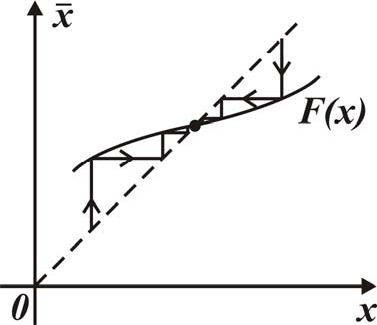
\includegraphics[width=\linewidth]{fig/lect6/5a}
                (a)
        \end{minipage}
        \begin{minipage}{0.49\linewidth}
                \centering
                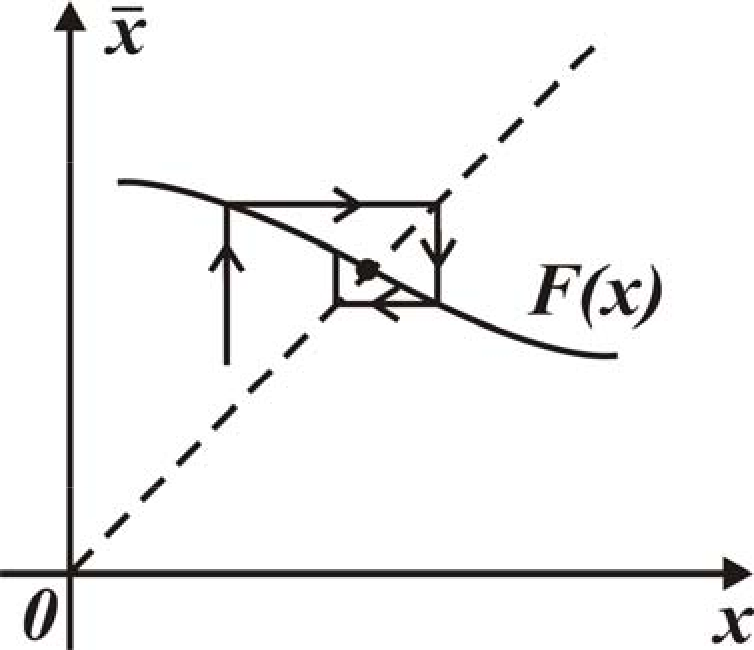
\includegraphics[width=\linewidth]{fig/lect6/5b}
                (b)
        \end{minipage}
        \begin{minipage}{0.49\linewidth}
                \centering
                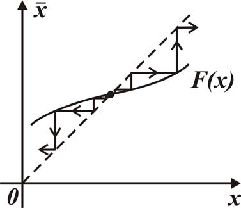
\includegraphics[width=\linewidth]{fig/lect6/5c}
                (c)
        \end{minipage}
        \begin{minipage}{0.49\linewidth}
                \centering
                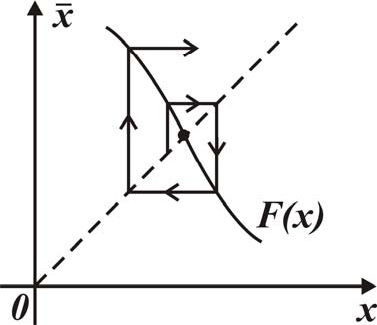
\includegraphics[width=\linewidth]{fig/lect6/5d}
                (d)
        \end{minipage}
        \caption{Диаграмма Ламерея для различных видов функции последования $F(x)$:
        в случае устойчивых неподвижных точек (a) и (b); в случай неустойчивых неподвижных
точек (c) и (d).}
        \label{fig:6.5}
\end{figure}
\begin{figure}[h]
        \centering
        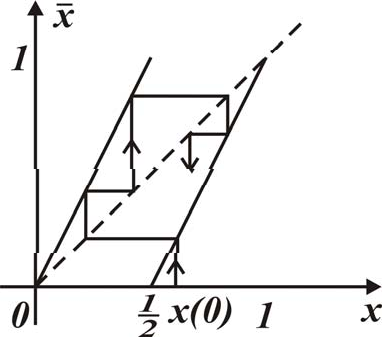
\includegraphics[width=0.6\linewidth]{fig/lect6/6}
        \caption{Отображение Бернулли и несколько его итерация начального условия $x(0)$}
        \label{fig:6.6}
\end{figure}
Нетрудно видеть, что отображение \eqref{eq:6.35} имеет две, отождествляемые между собой, неподвижные точки $x=0$ и $x=1$.
Покажем, что, несмотря на свой простой вид, отображений \eqref{eq:6.35} может демонстрировать сложную динамику.

Запишем начальное условие $x(0)$ в двоичной системе исчисления 
\begin{equation}
        \label{eq:6.36}
        x(0) = a_1,a_2,a_3,\dots,
\end{equation}
где $a_i \in \qty{0;1}$. В \eqref{eq:6.36} $a_1=0$, если $x(0) < \frac{1}{2}$ и
$a_1=1$, если $x(0) > \frac{1}{2}$.
Представление \eqref{eq:6.36} эквивалентно следующему
\begin{equation}
        \label{eq:6.37}
        x(0) = a_1 \cdot 2^{-1} + a_2 \cdot 2^{-2} + a_3\cdot 2^{-3}+\dots
\end{equation}
Используя \eqref{eq:6.37}, находим, что
\begin{equation}
        \label{eq:6.38}
        x(1) = 2x(0)= a_1 + a_2 \cdot 2^{-1}+a_3 \cdot 2^{-2}+ \dots
\end{equation}
и
\begin{equation}
        \label{eq:6.39}
        x(1) = 0, a_2,a_3\dots
\end{equation}
Ясно, что последующие итерации отображения \eqref{eq:6.36}  происходят по
аналогичному сценарию. Следовательно, действие отображения Бернулли на
двоичное представление $x$ сводится к удалению первого знака после запятой и
сдвигу оставшейся последующей последовательности влево. Это свойство
траекторий отображения \eqref{eq:6.35} называется \textbf{сдвигом Бернулли }. Используя это
свойство, покажем, что отображение \eqref{eq:6.35} может демонстрировать сложную
динамику.

Предположим, что двоичная последовательность \eqref{eq:6.36} является
периодической. Такой вид \eqref{eq:6.36} имеет место, если $x(0)$ -- рациональное число.
Поскольку каждое действие отображения \eqref{eq:6.35} сдвигу Бернулли,
то через некоторое число итераций, равное периоду двоичного кода
представления \eqref{eq:6.36}, переменная $x$ вернется в исходное состояние, Другими
словами, отображение \eqref{eq:6.35} имеет периодическую траекторию (цикл), период
которой равен периоду представления \eqref{eq:6.36}. С другой стороны, на единичном
интервале существует счетное множество рациональных чисел. Следовательно,
отображение \eqref{eq:6.35} имеет счетное множество циклов различного периода.
Например, пусть $x(0) = \frac{1}{3}$. В двоичной системе исчисления имеем следующую
динамику
\begin{align}
        x(0) = & 0,01010101 \dots \\
        x(1) = & 0,1010101 \dots \\
        x(2) = & 0,01010101 \dots \\
\end{align}
Следовательно, отображение \eqref{eq:6.35} имеет периодическую траекторию периода 2 или 2-цикл.
Рассмотрим две траектории отображения \eqref{eq:6.35}, стартующие с двух начальных условий $x(0)$ 
и $\tilde x(0)$,
различающихся лишь $(n+1)$ знака в представлении \eqref{eq:6.36},т.е. по крайней мере, $a_{n+1}\neq \tilde a_{n_1}$. Через $n$-итерация эти траектории будут иметь значения $F^n (x(0))$ и $F^n (\tilde x(0))$, которые будут отличаться уже в первом знаке.
Действительно, в силе действия сдвига Бернулли имеем
\begin{gather}
        F^n(x(0)) = 0 , a_{n+1}\dots \\
        F^n(\tilde x(0)) = 0, \tilde a_{n+1} \dots 
\end{gather}
Следовательно, траектории отображения \eqref{eq:6.35} обладают очень высокой чувствительностью
к начальным условиям, что характерно для хаотических движений.

Кроме рассмотренных здесь свойств, отображение \eqref{eq:6.35} обладает и другими, не менее интересными и сложными свойствами, которые мы обсудим позднее.


